\documentclass[11pt]{article}
\usepackage{amsmath,amsbsy,amssymb,verbatim,fullpage,ifthen,graphicx,bm,amsfonts,amsthm}
\usepackage{graphicx}
\usepackage{xcolor}
\newcommand{\mfile}[1]  {{\small \verbatiminput{./#1}}} % Jeff Fessler, input matlab file
\newcommand{\tmop}[1]{\ensuremath{\operatorname{#1}}}

\newcommand{\R}{\mathbb{R}}
\newcommand{\C}{\mathbb{C}}
\newcommand{\Z}{\mathbb{Z}}
\newcommand{\A}{\mathcal{A}}
\newcommand{\minimize}{\operatorname*{minimize\ }}
\newcommand{\maximize}{\operatorname*{maximize}}

%\newcommand{\mfile}[1]  {{\small \verbatiminput{./#1}}} 
\newcommand{\mtx}[1]{\mathbf{#1}}
\newcommand{\vct}[1]{\mathbf{#1}}
\def \lg       {\langle}
\def \rg       {\rangle}
\def \mA {\mtx{A}}
\def \mC {\mtx{C}}
\def \mI {\mtx{I}}
\def \mU {\mtx{U}}
\def \mS {\mtx{S}}
\def \mV {\mtx{V}}
\def \mW {\mtx{W}}
\def \mLambda {\mtx{\Lambda}}
\def \mX {\mtx{X}}
\def \mY {\mtx{Y}}
\def \mZ {\mtx{Z}}
\def \zero     {\mathbf{0}}
\def \vzero    {\vct{0}}
\def \vone    {\vct{1}}
\def \vu {\vct{u}}
\def \vv {\vct{v}}
\def \vx {\vct{x}}
\def \vy {\vct{y}}
\def \vz {\vct{z}}
\def \vphi {\vct{\phi}}
\def \vmu {\vct{\mu}}
\def \R {\mathbb{R}}


\usepackage{xspace}

\makeatletter
\DeclareRobustCommand\onedot{\futurelet\@let@token\@onedot}
\def\@onedot{\ifx\@let@token.\else.\null\fi\xspace}

\def\eg{\emph{e.g}\onedot} \def\Eg{\emph{E.g}\onedot}
\def\ie{\emph{i.e}\onedot} \def\Ie{\emph{I.e}\onedot}
\def\cf{\emph{c.f}\onedot} \def\Cf{\emph{C.f}\onedot}
\def\etc{\emph{etc}\onedot} \def\vs{\emph{vs}\onedot}
\def\wrt{w.r.t\onedot} \def\dof{d.o.f\onedot}
\def\etal{\emph{et al}\onedot} \def\st{\emph{s.t}\onedot}
\pagestyle{plain}

\title{{\bf Homework Set 1, CPSC 8420}}
\author{\Large\underline{LastName, FirstName}}
\date{\textbf{\Large\textcolor{red}{Due 10/07/2024, 11:59PM EST}}}

\begin{document}
\maketitle

\section*{Lasso}
As we discussed in class, one of the most efficient algorithm to find the optimal solution to Lasso is \textit{coordinate minimization} (also called alternating minimization) that every time we fix the rest while optimizing a certain coordinate until convergence.
\begin{equation}
	\frac{1}{2}\|Ax-y\|^2_2+\lambda\|x\|_1,
\end{equation}
Now, please randomly generate $A\in\R^{20\times10}, y\in \R^{20}$, and change $\lambda$ from $0.01$ to $1000$ with \textit{logspace}. You are expected to implement the codes with coordinate minimization method and the function should accept any $A,b, \lambda$ and return $x^*$. Compare the output with standard Lasso solver built in Matlab or python. And finally please plot the changes of $x$ with $\lambda$ varies. 

\vspace{4cm}

\section*{Least Squares Extension}
Assume $\mA, \mX, \mC, \mY, \mU \in\R^{n\times n}$. Given the fact that $vec(\mA\mU\mC)=(\mC^T\otimes\mA)vec(\mU)$, where $\otimes$ denotes \textit{Kronecker product}, please use \textit{least squares} we learned in class to solve:
\begin{equation}
	\min_\mX \|\mA\mX+\mX\mC-\mY\|_F^2.
\end{equation}
To verify the correctness of your solution: 1) randomly generate $\mA, \mX^*, \mC$; 2) set $\mY=\mA\mX^*+\mX^*\mC$; 3) by making use of least squares, you can obtain the optimal $vec(\mX)$ given $\mA, \mC, \mY$  and 4) compare with $vec(\mX^*)$.

\vspace{4cm}

\section*{Ridge Regression}
Please first conduct experiments to show that $\|(A^TA+\lambda\textbf{I})^{-1}A^Ty\|_2$ is a monotone (decreasing) function with respect to $\lambda$ (you may randomly generate $A, y$ and plot the objective changes with $\lambda$ increases). After you are pretty confident the argument is true, please prove it mathematically.

\vspace{4cm}

\section*{Linear Regression and its Extension}
\begin{figure}
	\centering
	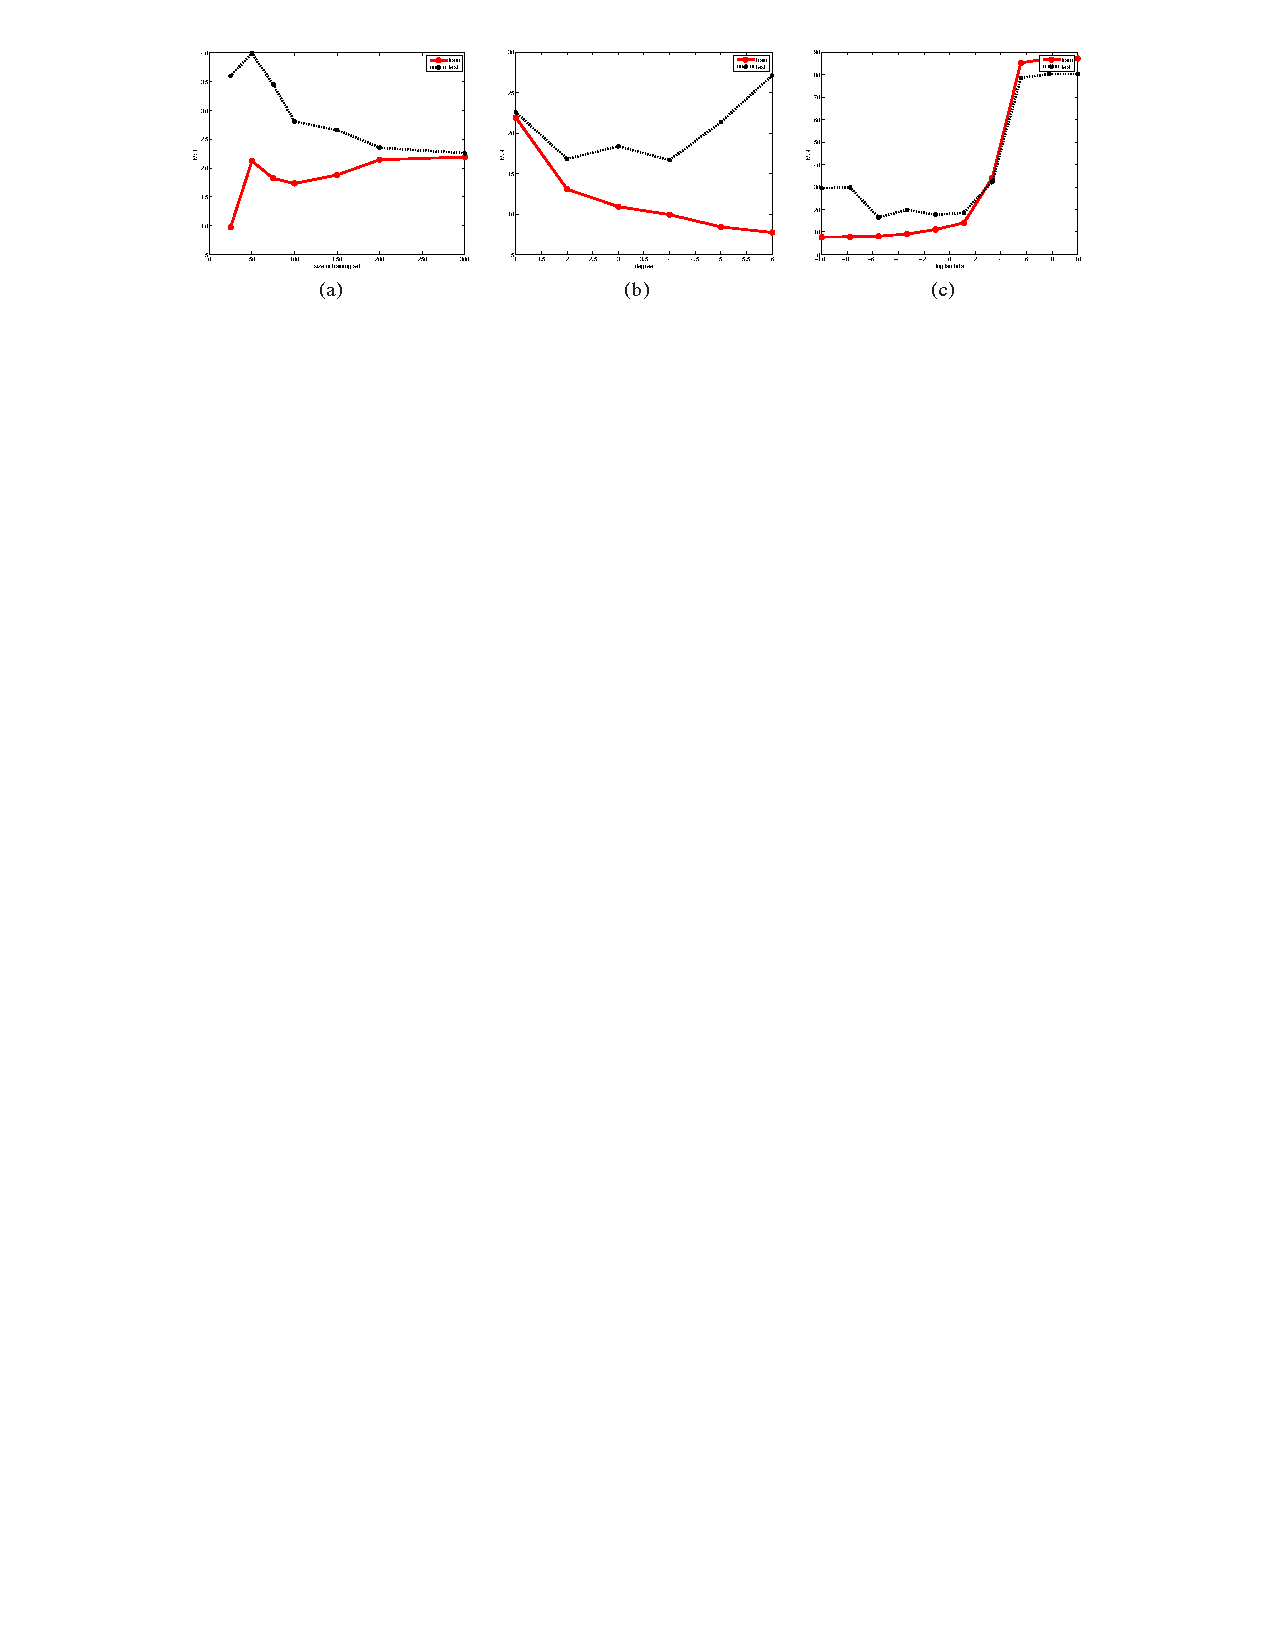
\includegraphics[width=1\linewidth]{fig}
	\caption{MSE vs (a) training set size, (b) polynomial degree, (c) size of ridge penalty. Solid Red = training, dotted black = test.}
	\label{fig:fig}
\end{figure}

In the Boston housing dataset, there are 506 records. We will
use first 13 features as inputs, $x$, and the 14th feature, median house price, as the output $y$. All features are continuous,
except feature 4, which is binary. However, we will treat this like any other continuous variable.
\begin{enumerate}
	\item Load the housing.data file. We will use the first 300 cases for training and the remaining 206 cases for
	testing. However, the records seem to be sorted in some kind of order. To eliminate this, we will shuffle the data
	before splitting into a training/test set. So we can all compare results, let use the following convention:
	\mfile{sample.m}
	\item Now extract the first n records of the training data, for $n \in \{25, 50, 75, 100, 150, 200, 300\}$. For each such
	training subset, standardize it (you may use \textit{zscore} function in Matlab), and fit a linear regression model using least squares. (Remember to include
	an offset term.) Then standardize the whole test set in the same way. Compute the mean squared error on
	the training subset and on the whole test set. Plot MSE versus training set size. You should get a plot like
	Figure 1(a). Turn in your plot and code. Explain why the test error decreases as n increases, and why the train
	error increases as n increases. Why do the curves eventually meet?
	As a debugging aid, here are the regression weights I get when I train on the first 25 cases (the first term is the
	offset, w0): $[26.11, -0.58, 3.02,\dots,-0.21, -0.27, -1.16]$.
	\item We will now replace the original features with an expanded set of features based on higher order terms. (We
	will ignore interaction terms.) For example, a quadratic expansion gives:
	\begin{equation}
		\begin{pmatrix}
			x_{11} & x_{12} & \dots & x_{1d} \\
			\vdots& \vdots & \ddots & \vdots \\
			x_{n1}& x_{n2} & \dots & x_{nd} \\
		\end{pmatrix}\xrightarrow[]{}\begin{pmatrix}
			x_{11} & x_{12} & \dots & x_{1d}& x_{11}^2 & x_{12}^2 & \dots & x_{1d}^2\\
			\vdots& \vdots & \ddots & \vdots&\vdots& \vdots & \ddots & \vdots \\
			x_{n1}& x_{n2} & \dots & x_{nd}& x_{n1}^2& x_{n2}^2 & \dots & x_{nd}^2\\
		\end{pmatrix}
	\end{equation}
The provided function degexpand(X,deg,addOnes) will replace each row of X with all powers up to degree deg. Use
this function to train (by least squares) models with degrees 1 to 6. Use all the the training data. Plot the MSE on
the training and test sets vs degree. You should get a plot like Figure 1(b). Turn in your plot and code. Explain
why the test error decreases and then increases with degree, and why the train error decreases with degree.
\item Now we will use ridge regression to regularize the degree 6 polynomial. Fit models using ridge regression with
the following values for $\lambda$:
$$lambdas=[0 \  logspace(-10,10,10)]$$
Use all the training data. Plot the MSE on the training and test sets vs $log_{10}(\lambda)$. You should get a plot like
Figure 1(c). Turn in your plot and code. Explain why the test error goes down and then up with increasing $\lambda$,
and why the train error goes up with increasing $\lambda$.
\end{enumerate}
\end{document}
